%                                                                 aa.dem
% AA vers. 9.1, LaTeX class for Astronomy & Astrophysics
% demonstration file
%                                                       (c) EDP Sciences
%-----------------------------------------------------------------------
%
%\documentclass[referee]{aa} % for a referee version
%\documentclass[onecolumn]{aa} % for a paper on 1 column  
%\documentclass[longauth]{aa} % for the long lists of affiliations 
%\documentclass[letter]{aa} % for the letters 
%\documentclass[bibyear]{aa} % if the references are not structured 
%                              according to the author-year natbib style

%
\documentclass{aa}  

%
\usepackage{graphicx}
%%%%%%%%%%%%%%%%%%%%%%%%%%%%%%%%%%%%%%%%
\usepackage{txfonts}
%%%%%%%%%%%%%%%%%%%%%%%%%%%%%%%%%%%%%%%%
%\usepackage[options]{hyperref}
% To add links in your PDF file, use the package "hyperref"
% with options according to your LaTeX or PDFLaTeX drivers.
%
\begin{document} 


   \title{Simulating the Universe from the Cosmic Microwave Background to Today}

   \subtitle{}

   \author{A. Martins
          \inst{1}
          }

   \institute{Institute of Theoretical Astrophysics, University of Oslo,
              Sem Sælands vei 13, 0371 Oslo\\
              \email{a.i.s.martins@astro.uio.no}
             }

   \date{}

% \abstract{}{}{}{}{} 
% 5 {} token are mandatory
 
  \abstract
  % context heading (optional)
  % {} leave it empty if necessary  
   {}
  % aims heading (mandatory)
   {}
  % methods heading (mandatory)
   {}
  % results heading (mandatory)
   {}
  % conclusions heading (optional), leave it empty if necessary 
   {}

   \keywords{
               }

   \maketitle
%
%-------------------------------------------------------------------

\section{Introduction}

\subsection{Background Cosmology}

\section{Theoretical Background}

\subsection{Background Cosmology}

We start by assuming that, at large scales, matter is homogeneous and isotropic. The mathematical formulation of this, i.e. the metric that describes the geometry of the Universe at large scales is given by the Friedmann–Lemaître–Robertson–Walker (FRLW) metric:
\begin{equation}
ds^2 = -dt^2 + a^2(t)(dx^2 + dy^2 + dz^2),
\end{equation}
where $a(t)$ is the scale factor of the Universe, a measure for the rate of its expansion.

We are interested in learning about the densities of the different components of the Universe at different points in time, from the Cosmic Microwave Background until the present day. The $\Lambda$CDM model assumes that the Universe is composed of matter (baryons\footnote{Baryons in this context refers to all "normal" matter, i.e. quarks, leptons (not including neutrinos for our purposes) and combinations of them.} and cold, dark matter), radiation (photons and neutrinos) and dark energy. Another important notion for our model is that of curvature, which we already implicitly assumed to be 0 in the above equation, i.e. we are assuming a flat Universe. These components come together in the Friedman equation, which relates their density evolution to the expansion of the Universe:
\begin{equation}
H(a) = H_0 \sqrt{\Omega_{M0}a^{-3} + \Omega_{R0}a^{-4} + \Omega_{k 0} a^{-2} + \Omega_{\Lambda 0}},
\end{equation}
where $H(a)$ is the so-called Hubble parameter and $H_0$ is the Hubble constant, measured experimentally today to be around 68.3 km s$^{-1}$ Mpc$^{-1}$ \citep{Kozmanyan_2019}. Each $\Omega_{i0}$ represents the density of one of the above-mentioned components in the present day, now explicitly including curvature $k$, and $\Omega_{M0} = \Omega_{b0} + \Omega_\text{CDM0}, \Omega_{R0} = \Omega_{\gamma0} + \Omega_{\nu0}$. The densities for photons and neutrinos today are given by
\begin{align}
\Omega_{\gamma 0} &= 2\cdot \frac{\pi^2}{30} \frac{(k_bT_{\rm CMB 0})^4}{\hbar^3 c^5} \cdot \frac{8\pi G}{3H_0^2},\\
\Omega_{\nu 0} &= N_{\rm eff}\cdot \frac{7}{8}\cdot \left(\frac{4}{11}\right)^{4/3}\Omega_{\gamma 0},
\end{align}
whereas the densities for baryons and cold, dark matter are assumed to be, respectively, 0.05 and 0.267, the values given by \cite{2020}. The densities of all the components need to, of course, add up to one. We then find that 
$\Omega_{\Lambda 0} = 1 - (\Omega_{b 0}+\Omega_{\rm CDM 0}) - (\Omega_{\gamma 0} + \Omega_{\nu 0}) - \Omega_{k 0}$, where, assuming a flat universe, $\Omega_{k 0} = 0$.

We can get the component densities for different scale factors from
\begin{equation}
\label{eq:omegas}
\begin{aligned}
\Omega_{k}(a) &= \frac{\Omega_{k0}}{a^2H(a)^2/H_0^2}\\
\Omega_{\rm CDM}(a) &= \frac{\Omega_{\rm CDM 0}}{a^3H(a)^2/H_0^2} \\
\Omega_b(a) &= \frac{\Omega_{b 0}}{a^3H(a)^2/H_0^2} \\
\Omega_\gamma(a) &= \frac{\Omega_{\gamma 0}}{a^4H(a)^2/H_0^2} \\
\Omega_{\nu}(a) &= \frac{\Omega_{\nu 0}}{a^4H(a)^2/H_0^2} \\
\Omega_{\Lambda}(a) &= \frac{\Omega_{\Lambda 0}}{H(a)^2/H_0^2}.
\end{aligned}
\end{equation}

It is handy to explore the Hubble parameter equations before introducing some new notions. In particular, a useful quantity is the scaled Hubble parameter $\mathcal H = aH$. Deriving this with respect to $x = \log a$ and denoting the derivative with respect to $x$ as ', we have
\begin{align}
    \mathcal H' &= \frac{d\mathcal H}{dx} = \frac{da}{dx}\frac{d\mathcal H}{da}\\ 
    &= a\left( H(a) + \frac{1}{2}\frac{aH_0^2}{ H(a)} (-3\Omega_{M0} a^{-4} - 4\Omega_{R0}a^{-5}-2\Omega_{k0}a^{-3})\right)\\
    &= \mathcal H(x) +\frac{1}{2}\frac{(e^xH_0)^2}{\mathcal H(x)}(-3\Omega_{M0} e^{-3x} - 4 \Omega_{R0}e^{-4x}-2\Omega_{k0}e^{-2x}).
\end{align}

Deriving once more, we get
\begin{alignat*}{2}
    \mathcal H'' &= \frac{d^2\mathcal H}{dx^2}&&\\ 
    &= \mathcal H'\Bigg(1-&&\frac{1}{4}\left(\frac{e^xH_0}{\mathcal H(x)}\right)^5\\
    & &&(3\Omega_{M0}e^{-3x}+4\Omega_{R0}e^{-4x}+2\Omega_{k0}e^{-2x})^2\\
    & &&(9\Omega_{M0}e^{-3x}+16\Omega_{R0}e^{-4x}+4\Omega_{k0}e^{-2x})\Bigg)
\end{alignat*}

It is now useful to define the notion of conformal time $\eta$, the distance the light has traveled since the Big Bang, taking into account the expansion of the Universe. A differential equation for $\eta$ can be written as
\begin{align}
\frac{d\eta}{dx} = \frac{da}{dx}\frac{d\eta}{da} = \frac{c}{\mathcal{H}}.
\end{align}

From this, follow the definition of the co-moving distance $\chi$, the distance between the observer and a measurable quantity:
\begin{align}
\chi = \eta_0 - \eta
\end{align}

For a flat Universe, we can define the luminosity distance, i.e. given the intrinsic luminosity of a source and its flux, the distance to the source is

\begin{equation}
    d_L = \frac{\chi}{a}.
\end{equation}

A last useful notion before we get into some deductions is that of cosmic time $t$, which is given by solving
\begin{align}
\label{eq:t-ode}
\frac{dt}{dx} = \frac{1}{H}.
\end{align}

We are now interested in looking at specific points in time, such as the points when matter and radiation had the same density and when matter and dark energy had the same density (and subsequent dominating periods), and the time when the Universe started to accelerate.

\subsubsection{Matter-Radiation Equality}

We can find the time of matter-radiation equality by equating $
\Omega_b + \Omega_{\rm CDM} = \Omega_\gamma + \Omega_{\nu}$. Using \eqref{eq:omegas}, we find that

\begin{equation}
    a = \frac{\Omega_R}{\Omega_M}.
\end{equation}

\subsubsection{Matter-Radiation Equality}

Similarly, we find the time when matter and radiation are equally dense by equating $\Omega_b + \Omega_{\rm CDM} = \Omega_{\Lambda}$ and find that

\begin{equation}
    a = \sqrt[3]{\frac{\Omega_M}{\Omega_{\Lambda}}}
\end{equation}

\subsubsection{The Universe starts to accelerate}

In order to know when the Universe starts to accelerate, we must solve $\ddot a = 0$. By definition, $H = \dot{a}/a \Rightarrow \frac{d}{dt} \dot a = \frac{d}{dt} (aH) = \frac{d}{dt}\mathcal H$. It is not so useful to take the derivative in terms of cosmic time of the scaled Hubble parameter, but we already know what its derivative is in terms of $x$, so we can take that and get
\begin{equation}
    \ddot a = \frac{dx}{dt}\frac{d\mathcal H}{dx},
\end{equation}
where we know a handy expression for $\frac{dx}{dt}$ from \eqref{eq:t-ode} and we end up with
\begin{equation}
    \ddot a = H\mathcal{H'} = 0,
\end{equation}
where ' denotes the derivative in terms of $x$.

\section{Implementation, numerical methods and tests}

\subsection{Background Cosmology}

We now want to use the previously presented equations in order to compute the relevant quantities over different scale factors. The code to reproduce this simulation is available at \url{https://github.com/anaismartins/AST5220-Cosmology}. For more readable but still fast calculations, these were written in Python (\texttt{src\\python}) with equations ported from C++ (\texttt{src\\cpp}) using \texttt{ctypes} \cite{ctypes}.

\subsubsection{Solving ODEs}

In particular, we have two important quantities defined by ordinary differential equations (ODEs), the conformal time $\eta$ and the cosmic time $t$. In order to solve them, we use a fourth order Runge-Kutta method, followed by splining the results over a relevant range, which, in our case, was chosen to be from $x=\log(10^{-8})$ until today ($x=0$).

\subsubsection{Markov Chain Monte Carlo Sampling}

We are interested in finding the value of the Hubble constant $H_0$, as well as the densities of the components of the Universe. To do this, we run a Markov chain Monte Carlo method, sampling $h = \frac{H_0}{100\text{ km s}^{-1}\text{ Mpc}^{-1}}$ (the dimensionless Hubble constant), $\Omega_M$ and $\Omega_k$ from data from supernova type IA observations \citep{Betoule_2014}.

\section{Results}

\subsection{Background Cosmology}

According to our simulations, the densities of the different components of the Universe evolve as shown in Figure \ref{fig:Omegas}. This results in the scaled Hubble parameter shown in Figure \ref{fig:Hp}. The vertical lines in each of these figures represent relevant points in time, and the values for each of these are shown in Table \ref{table:times}. The analytical calculations that give the values in the table seem to agree with the curves derived from simulations in the figures, demonstrating trustworthy results.

\begin{figure}[ht]
\centering
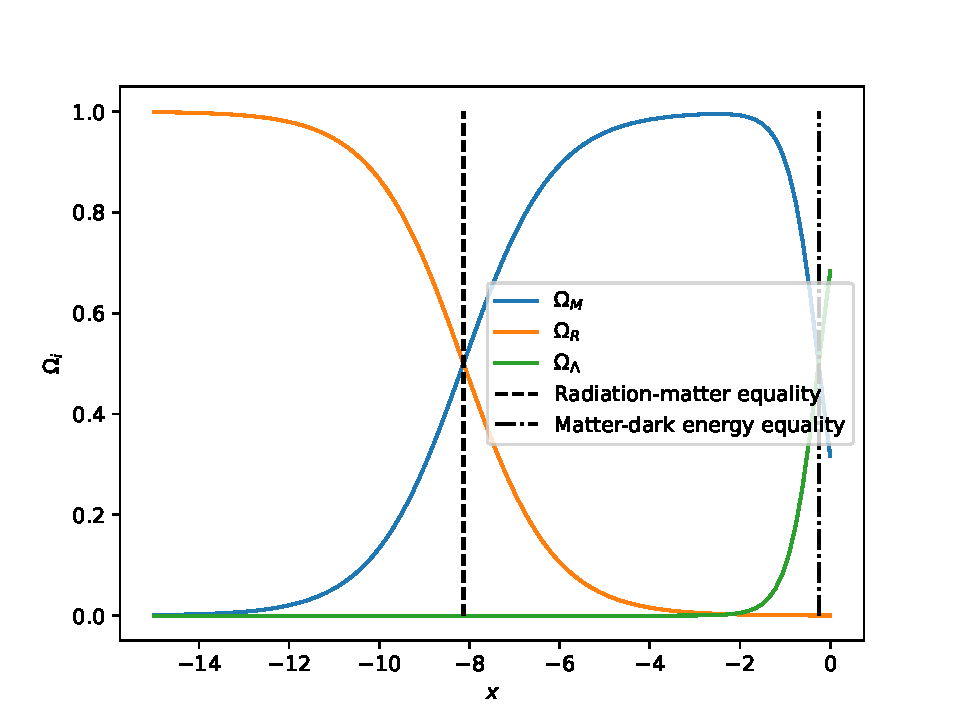
\includegraphics[width=\hsize]{figures/Omegas.pdf}
  \caption{Evolution of the densities of the components of the Universe as a function of the logarithm of the scale factor, where the density of matter, radiation and dark energy are shown, respectively, in blue, orange and green. The black vertical lines show the radiation-matter (dashed) and matter-dark energy (dot-dashed) equalities. In the beginning, radiation dominates; in between the two vertical lines, matter dominates; and, closer to today, dark energy dominates.}
     \label{fig:Omegas}
\end{figure}

\begin{figure}[ht]
\centering
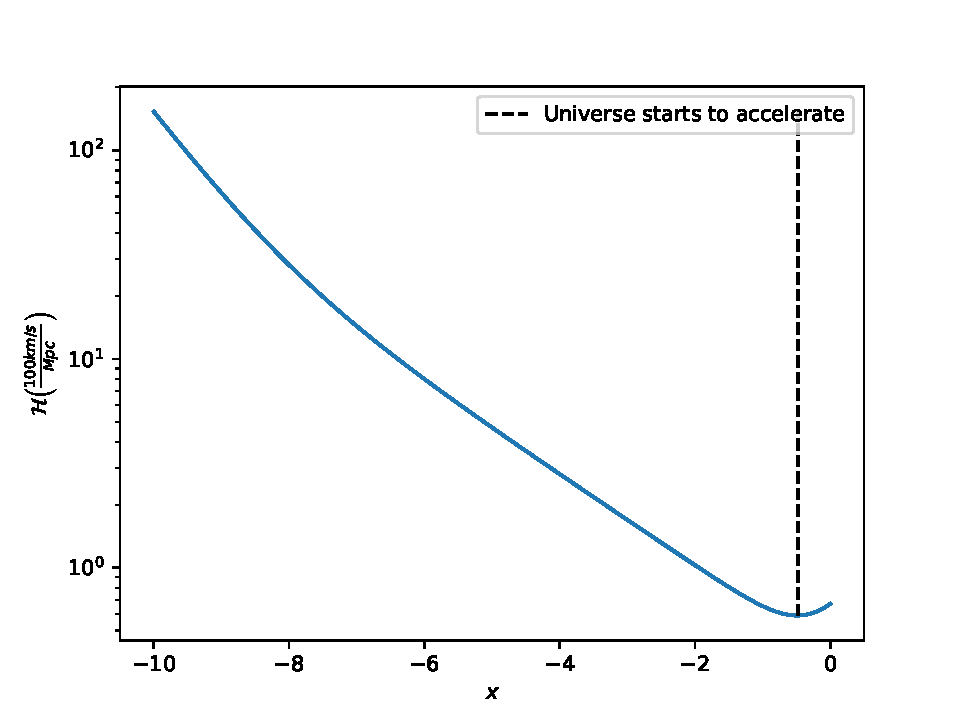
\includegraphics[width=\hsize]{figures/Hp.pdf}
  \caption{Scaled Hubble parameter as a function of the logarithm of the scale factor (blue). The black vertical dashed line represents the point where the Universe starts to accelerate.}
     \label{fig:Hp}
\end{figure}

\begin{table*}[ht]
\caption{Nonlinear Model Results}             
\label{table:times}      
\centering          
\begin{tabular}{l l l l}     % 7 columns 
\hline\hline       
                      % To combine 4 columns into a single one 
& Logarithm of scale factor $x$      & Redshift $z$     & Cosmic time $t$ (Gyr)\\ 
\hline                    
Radiation-Matter Equality   & -8.1319  & 3400.3  & 5.1029 $\times 10^{-5}$ \\
Matter-Dark Energy Equality & -0.25582 & 0.29152 & 10.371                 \\
Universe starts to accelerate ($\ddot a = 0$)               & -0.47941 & 0.61513 & 7.8234\\ 
\hline                  
\end{tabular}
\end{table*}

We can also see 

The conformal time of today ($a = 1 \Rightarrow x = 0$) is 14.192 Gpc.

\begin{figure}[ht]
\centering
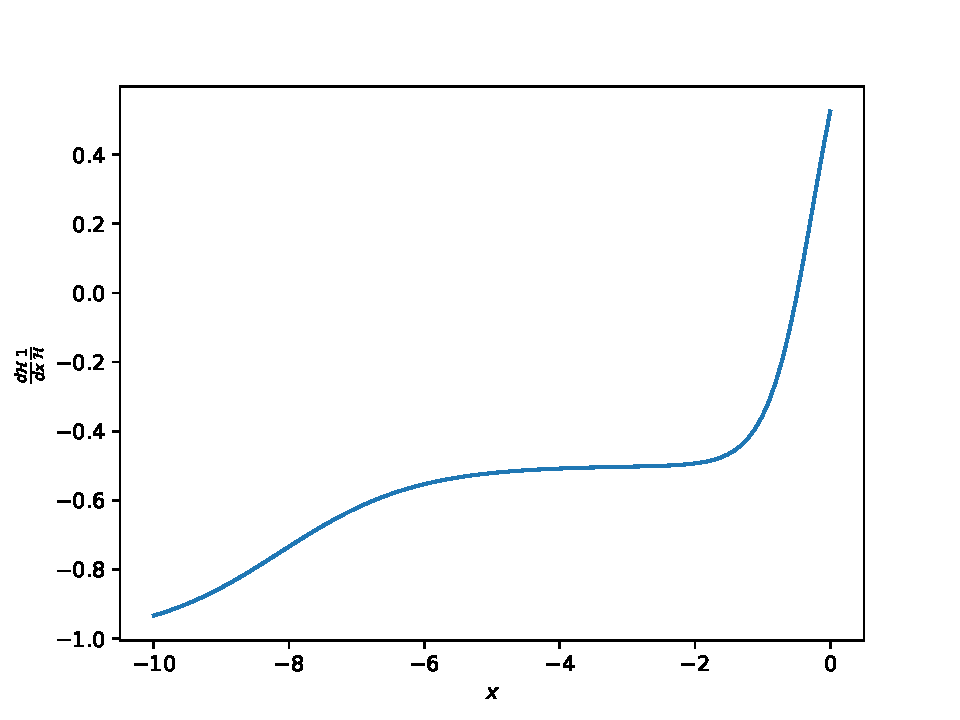
\includegraphics[width=\hsize]{figures/dHpdx_over_Hp.pdf}
  \caption{}
     \label{}
\end{figure}

\begin{figure}[ht]
\centering
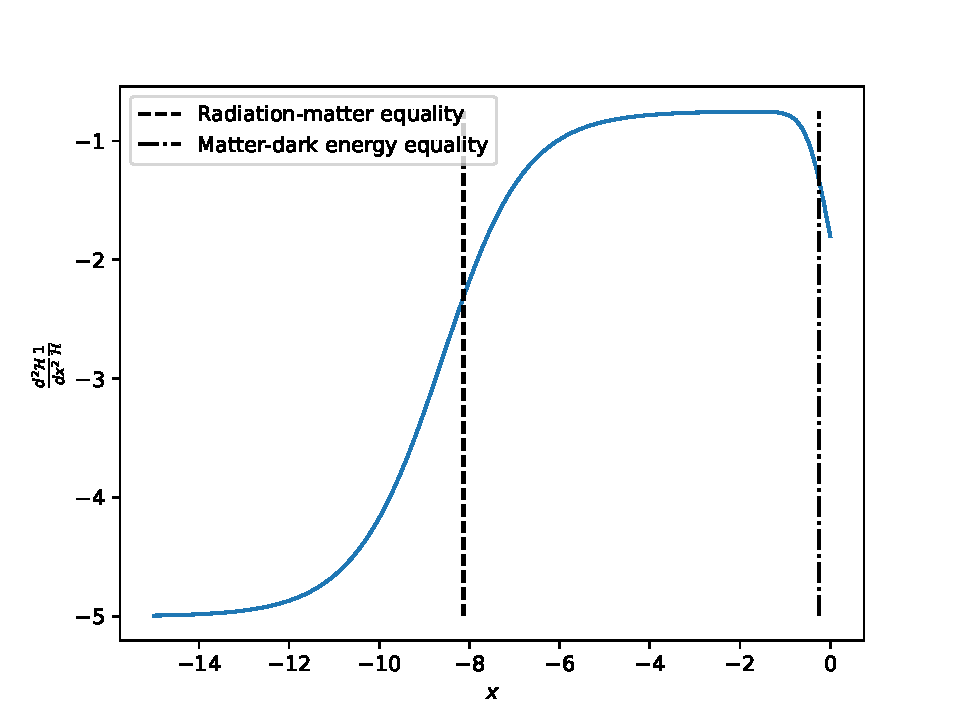
\includegraphics[width=\hsize]{figures/ddHpddx_over_Hp.pdf}
  \caption{}
     \label{}
\end{figure}

\begin{figure}[ht]
\centering
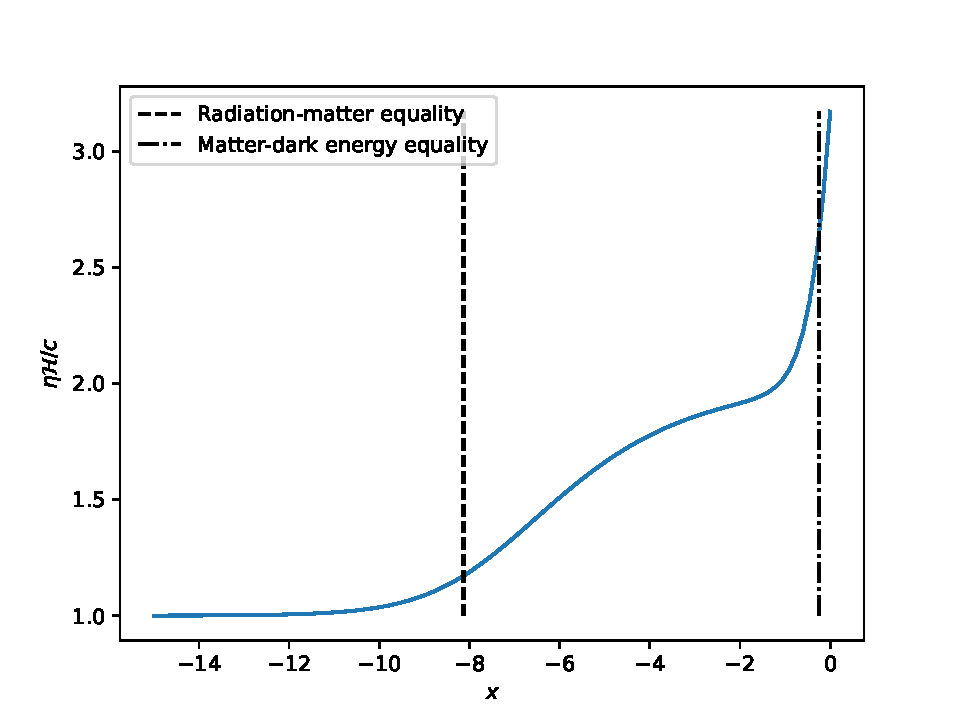
\includegraphics[width=\hsize]{figures/etaHp_over_c.pdf}
  \caption{}
     \label{}
\end{figure}

\begin{figure}[ht]
\centering
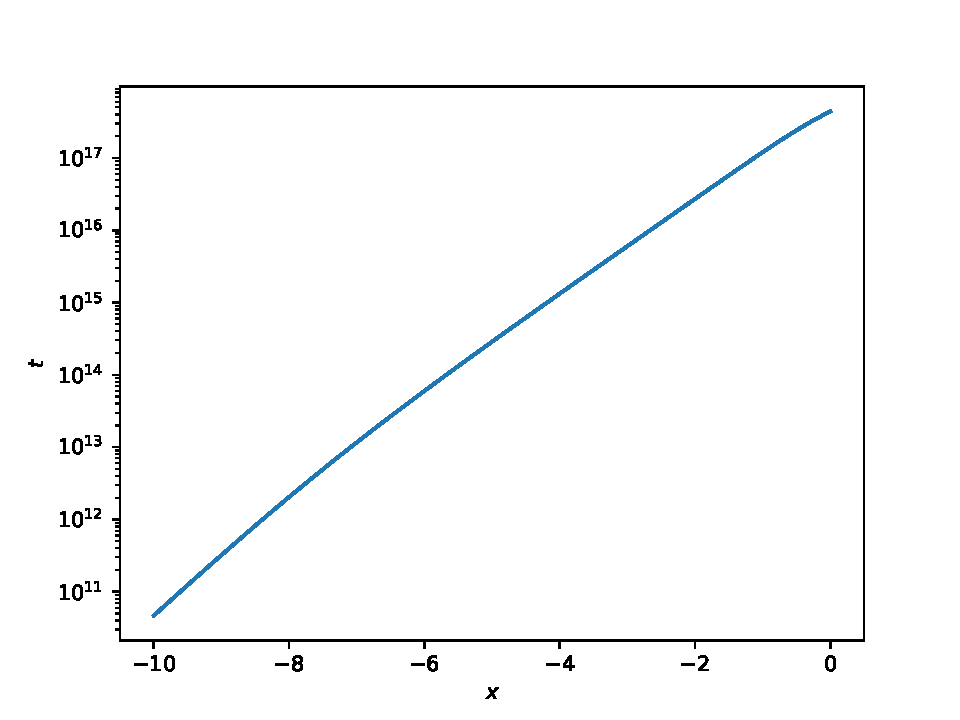
\includegraphics[width=\hsize]{figures/t.pdf}
  \caption{}
     \label{}
\end{figure}

\begin{figure}[ht]
\centering
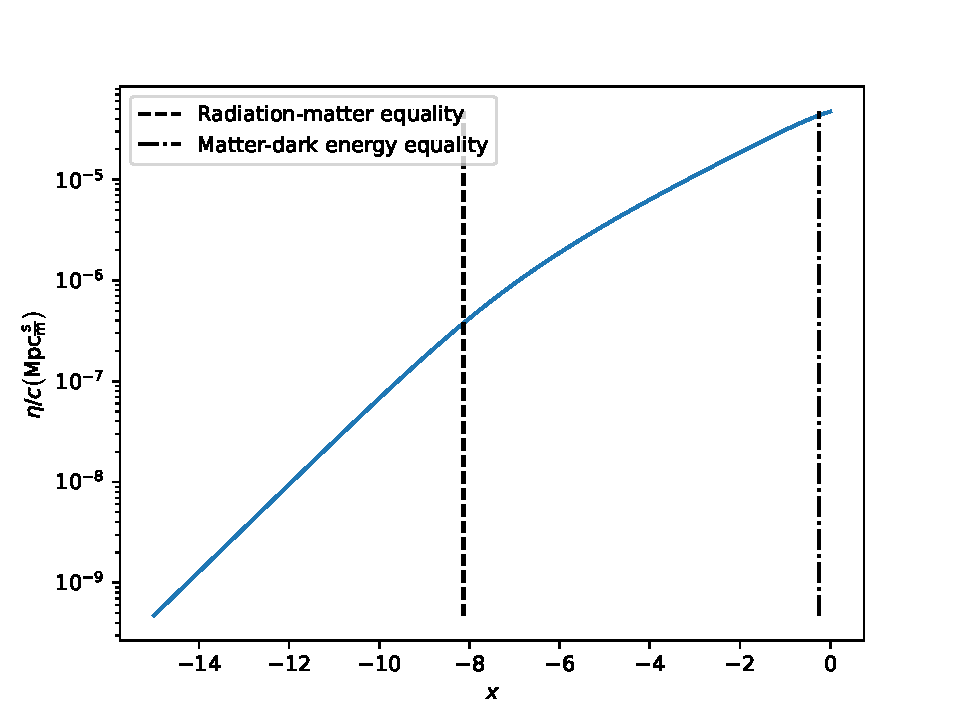
\includegraphics[width=\hsize]{figures/eta_over_c.pdf}
  \caption{}
     \label{}
\end{figure}

\begin{figure}[ht]
\centering
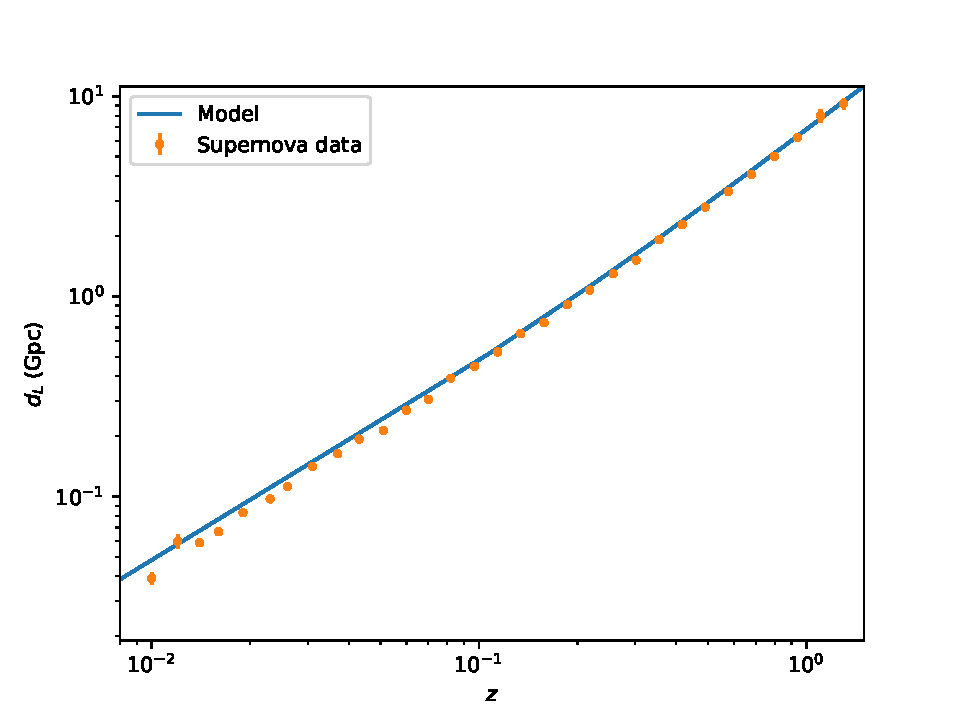
\includegraphics[width=\hsize]{figures/dL.pdf}
  \caption{}
     \label{}
\end{figure}

\begin{figure}[ht]
\centering
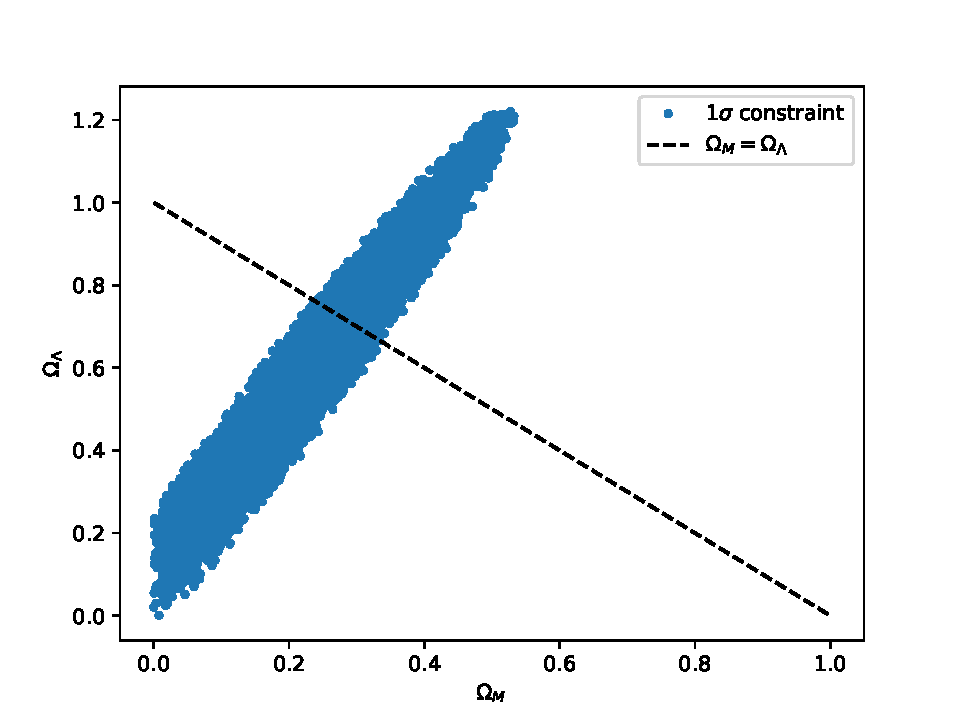
\includegraphics[width=\hsize]{figures/fitting.pdf}
  \caption{}
     \label{}
\end{figure}

\begin{figure}[ht]
\centering
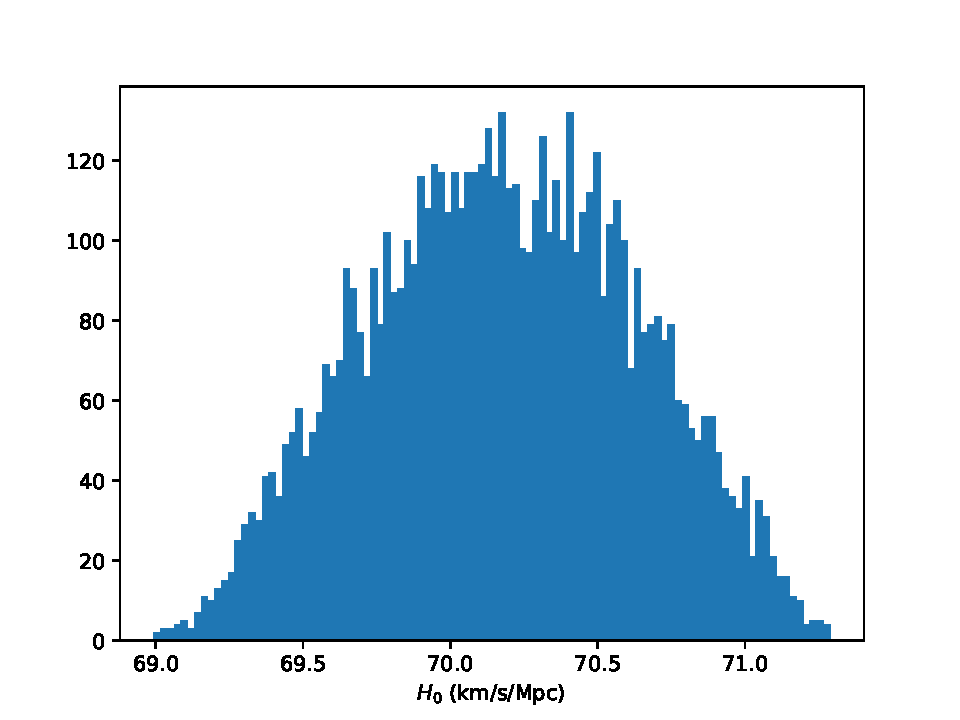
\includegraphics[width=\hsize]{figures/histogram.pdf}
  \caption{}
     \label{}
\end{figure}



\section{Conclusions}

\subsection{Background Cosmology}

\begin{acknowledgements}

\end{acknowledgements}

% WARNING
%-------------------------------------------------------------------
% Please note that we have included the references to the file aa.dem in
% order to compile it, but we ask you to:
%
% - use BibTeX with the regular commands:
%   \bibliographystyle{aa} % style aa.bst
%   \bibliography{Yourfile} % your references Yourfile.bib
%
% - join the .bib files when you upload your source files
%-------------------------------------------------------------------

\bibliographystyle{aa}
\bibliography{report/references}

\end{document}
